\documentclass[10pt]{article}
\usepackage[margin=0.7in]{geometry}
\usepackage{times}
\usepackage{mathptmx}
\usepackage{graphicx}
\usepackage[colorlinks=true,urlcolor=blue]{hyperref}
\setlength{\parindent}{0pt}
\setlength{\parskip}{6pt}
\pdfcompresslevel=9
\pdfobjcompresslevel=3
\begin{document}
\begin{center}
{\Large Native cubic-transfer follow-up}\\[4pt]
2026-10-25 \quad Synthetic public fixtures; partial research results
\end{center}

\textbf{Requested scope.} Prove or disprove one additional degree-three
isogeny after torsion preparation; complete exceptional-chart handling;
run isolated repeated end-to-end benchmarks. All three remain partial.
Historical Sage evidence is preserved unchanged.

\textbf{A symbolic result.} In characteristic other than two or three, set
$u=3s^2$, $m=3s$, $a=6sv-27s^4$ and
$b=v^2-18s^3v+54s^6$. For $v\ne0$ and $v\ne4s^3$,
$P=(u,v)$ is three-torsion on $y^2=x^3+ax+b$. In the row basis
$(1,x,y)$, its normalized translation lift is $M=N/(2v)$, with
\[
N=\left(\begin{array}{ccc}
mu-v & mu^2-3uv & 3v^2-umv\\
-m & 2v-mu & mv\\
-1 & -u & -v
\end{array}\right).
\]
Native exact integer polynomial expansion checks $M^3=I$, the rational
translation formula after denominators are cleared, and
$4a^3+27b^2=27v^3(v-4s^3)$. The existing Rust checker replays the
certificates with 64 extra points and false-identity rejection controls.
The formula matches all 232 nonzero torsion actions on 29 saved fixtures.
This is a rational formula for a standard theta-group construction;
novelty is not claimed. It does not settle neighboring obstruction signs.

Translation certificate: \texttt{IDC1ha43e239b427420d9}.\\
Order certificate: \texttt{IDC1hf37d8dfb82d48731}.\\
Discriminant certificate: \texttt{IDC1hdfe4817e960b55ff}.
These are evaluated records plus exact coefficient calculations, not Lean proofs.

\textbf{Geometric chart availability.} Assume a smooth plane quartic has
$N_1=p+1$, $N_2=p^2+1$, prime Jacobian order $r$, and
$r\ge p^3+1-2p^{3/2}$. Its symmetric square has $p^2+p+1$ rational points.
Special degree-three classes contribute at most $p+1$ bad classes;
nonreduced divisors at most $(p+1)^2$; support on a fixed infinity line
at most $4(p^2+p+1)$. Hence at most $B=5p^2+7p+6$ classes lack a
unique reduced affine representative. For three nonzero group elements,
at most $3B$ common multipliers fail. For $p\ge19$, $r-1>3B$.
The positivity calculation is certificate \texttt{IDC1h6cc11bdc8a4651a3}.

This is an agent-derived geometric argument, not an independently reviewed
formal proof. It does not establish that the present forward formulas or
polynomial inverter work everywhere in that domain. Native projective
local-jet recovery checks all 64, 568 and 1,860 rational effective
degree-three divisors on the declared test curves at $p=5,7,11$.
It starts from support coordinates; it is not a Kummer-image inverter.

\newpage
\textbf{Repeated native diagnostics.} Five seeds per arm and prime give
50 main runs, plus eight A/A repeats. All 58 recover correct scalars;
A/A counted outputs match. A separate FLINT implementation checks all
answers on the original source curves. Target points are synthetic on the
fixed historical quartics and share the known answer; a native forward
map has not been executed.

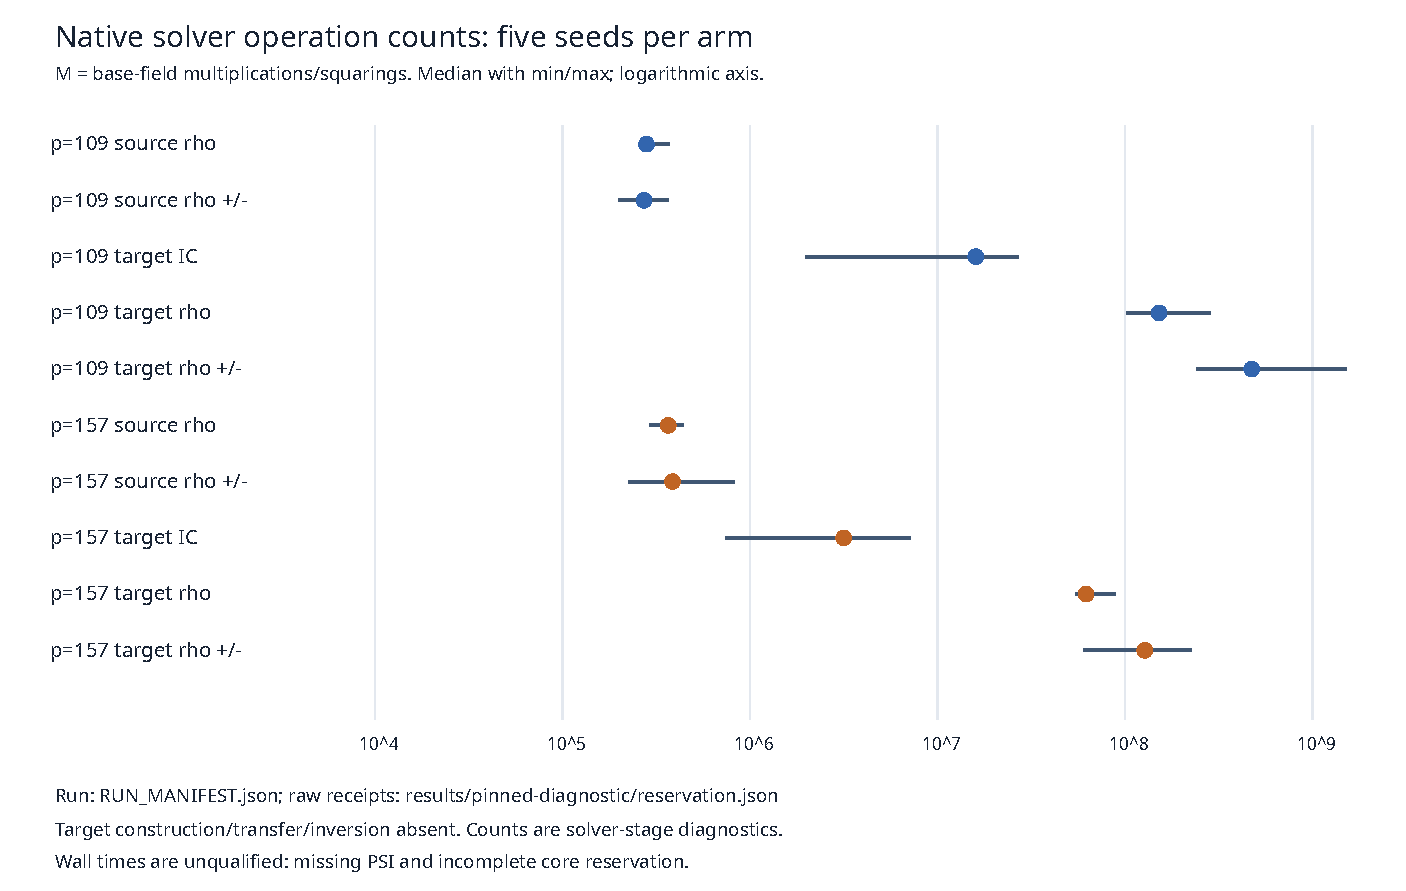
\includegraphics[width=\linewidth]{../results/native-counts.pdf}

\begin{center}\small
\begin{tabular}{r l r r}
$p$ & Arm (five seeds) & Median $M$ & Median $I$\\\hline
109 & Source rho & 280,521 & 3,532\\
109 & Source rho with negation & 272,286 & 3,237\\
109 & Target index calculus & 16,001,836 & 667,005\\
109 & Target rho & 151,955,436 & 6,339,785\\
109 & Target rho with negation & 474,000,284 & 19,769,067\\
157 & Source rho & 366,579 & 4,823\\
157 & Source rho with negation & 386,379 & 4,583\\
157 & Target index calculus & 3,160,099 & 129,612\\
157 & Target rho & 61,989,685 & 2,567,482\\
157 & Target rho with negation & 127,470,615 & 5,284,059
\end{tabular}\end{center}

\textbf{No qualified wall times.} Strict preflight refuses missing CPU
and memory PSI. Diagnostic workers are pinned to CPU 3, with an exclusive
lock and 16 movable threads evicted, but system threads remain eligible.
No visible-tick contention is detected; this does not repair incomplete
reservation or missing pressure metrics. Raw unqualified wall times,
context switches, faults, RSS and A/A spread are retained.

\newpage
\textbf{The exact remaining mathematical obligation.} Label the twelve
obstructions and eligible neighbors on the relevant level-nine moduli
strata. Compute the obstruction functions' divisors modulo two and the
arithmetic square classes of constants. A relation
$\prod u_i^{e_i}=c w^2$ excludes the all-negative star precisely when
$\sum e_i$ disagrees with the character bit of $c$.
The two saved bad centers have nonsquare neighbor products, but this
does not establish a universal identity. The rational translation lift
removes one interpolation dependency; neighbor labelling and modular
divisor calculations remain open.

\textbf{Evidence entry points.} Paths are relative to this report:
\href{../PROTOCOL.md}{PROTOCOL.md};
\href{../RUN_MANIFEST.json}{RUN\_MANIFEST.json};
\href{../results/pinned-diagnostic/reservation.json}{raw reservation and job receipts};
\href{../results/benchmark-summary.json}{benchmark summary};
\href{../results/source-replay.json}{FLINT scalar replay};
\href{../results/theta-symbolic-audit.json}{symbolic theta audit};
\href{../results/theta-certificate-replay.json}{theta certificate replay};
\href{../results/certificate-replay.json}{other certificate replay};
\href{../results/normalization-family-audit.json}{normalization compatibility};
\href{../GEOMETRIC_CHART_BOUND.md}{geometric argument};
\href{../SQUARE_CLASS_OBLIGATION.md}{square-class obligation};
\href{../results/development-obstructions.json}{failed attempts and open gaps}.

The source and binary hashes are in
\href{../results/benchmark-input-sha256.txt}{benchmark-input-sha256.txt};
the worker hash begins \texttt{8c67ce79c66ac501}. Run identity is the
manifest hash beginning \texttt{4dc7f9aab3f92759}. UTC process-start
timestamps were not captured; filesystem times are not substituted.
Compiler and host records sit in results/. No historical Sage timing is
combined with these observations.

\textbf{Validation and publication limits.} Standalone quartic/source
tests pass on both fixtures, native C++ tools build with warnings as errors,
and six polynomial certificates pass the existing Rust checker. Same
host/session arithmetic checks do not constitute independent-host replay.
The root release-test command cannot run in the partial import checkout
because Cargo.toml is absent. Conductor, Lean/Lake and five original S3
uploads remain unresolved. Full native construction, inversion, matched
isolation, external comparison and calibrated accounting are not complete.

Historical component figures are unchanged: no new coverage edge was
found. The scoreboard, registry, benchmark index and leaderboard are
unchanged. A browsing copy of this report and graph is included under:
\par\texttt{benchmarks/}\\
\texttt{20261025-cubic-transfer-native-diagnostics/}.
There is no admitted performance row and no full-pipeline speedup claim.

\textbf{Prior methods.} Tian, \href{https://arxiv.org/abs/2012.07173}{Cover
Attacks for Elliptic Curves}; algebraic obstruction methods,
\href{https://arxiv.org/abs/2004.08315}{Kirschmer et al.}; geometric
index calculus, \href{https://members.loria.fr/EThome/files/non-he-genus3.pdf}{Diem--Thome}.
The native quartic arithmetic is pinned from repository PR \#2170.
\end{document}
